\documentclass[14pt,a4paper]{extreport}
% preamble.tex — спільна преамбула для всіх лабораторних робіт. Підключається одразу після \documentclass у кожному lab*/main.tex.
%
% ЗБІРКА: LuaLaTeX (не pdfLaTeX). Причина: пакет listings під pdfLaTeX не читає UTF-8 і зупиняє збірку на кириличних коментарях у лістингах програмного коду. LuaLaTeX обробляє UTF-8 нативно.
%
% ШРИФТ: Liberation Serif — метрично сумісний з Times New Roman і містить повний набір кириличних гліфів (TeX Gyre Termes кирилиці не має, через що український текст не відображався взагалі).

\usepackage{fontspec}
\setmainfont{Liberation Serif}
\setmonofont{DejaVu Sans Mono}[Scale=0.82]

\usepackage{polyglossia}
\setmainlanguage{ukrainian}
\setotherlanguage{english}

\usepackage{microtype}

% Поля, інтервал, відступи й заголовки нижче взяті з шаблону НУЛП, за яким написана бакалаврська робота (../bachelor-thesis/thesis/main.tex). Той самий формат приймає В.М. Шиманський і для магістерських, тож усі звіти тримаємо в ньому, а не в тому, що переказували на консультації.
\usepackage[left=25mm,right=15mm,top=15mm,bottom=23mm,footskip=1.5mm]{geometry}
\usepackage{setspace}
% Саме \setstretch{1.5}, а не \onehalfspacing: останній дає близько 1.25.
\setstretch{1.5}

\usepackage{graphicx}
\usepackage{float}
\usepackage{booktabs}
\usepackage{array}
\usepackage{tabularx}
\usepackage{longtable}
\usepackage{enumitem}
% labelindent вирівнює маркер списку з абзацним відступом — так у шаблоні НУЛП.
\setlist{nosep}
\setlist[itemize]{label=\textbullet,leftmargin=*,labelindent=1.27cm}
\setlist[enumerate]{leftmargin=*,labelindent=1.27cm}
\usepackage{indentfirst}
\usepackage{amsmath}

\usepackage{hyperref}
\hypersetup{colorlinks=true,linkcolor=black,urlcolor=blue,citecolor=black}

% xurl дозволяє \url розривати адресу в будь-якому місці, а не лише після скісної риски. Без нього довгий сегмент шляху (напр. «scopus---podrobnaya- instruktsiya-dlya-uchenogo») виходить за межі сторінки, бо дефіс для hyperref не є точкою розриву. Вантажиться після hyperref — перевизначає його \UrlBreaks.
\usepackage{xurl}

% ---------------------------- Лістинги програмного коду ---------------------------- Використано minted (через Pygments), а не listings: listings не вміє коректно обробляти багатобайтові символи й «висмикує» кириличні коментарі з коду, зліплюючи їх в один рядок. Потребує прапорця -shell-escape.
\usepackage{xcolor}
\usepackage[newfloat]{minted}
% labelsep=period дає «Рис. 2.1. Назва» замість «Рис. 2: Назва» — формат НУЛП.
\usepackage[labelsep=period]{caption}

% baselinestretch=1 обов'язковий: без нього лістинг успадковує півторашку основного тексту, і довгий фрагмент коду перестає вміщатися у сторінку. Усередині [H]-флоата це не помилка збірки, а нескінченний цикл порожніх сторінок — lab1 так намолотив 161 тисячу сторінок.
\setminted{
  baselinestretch=1,
  fontsize=\footnotesize,
  linenos=true,
  frame=single,
  framesep=4pt,
  breaklines=true,
  breakanywhere=true,
  tabsize=4,
  numbersep=7pt,
  bgcolor=gray!8,
}
\setminted[python]{python3=true}

\SetupFloatingEnvironment{listing}{name=Лістинг,listname=Перелік лістингів}

% ---------------------------- Нумерація та оформлення заголовків ----------------------------
\usepackage{titlesec}

\setcounter{secnumdepth}{3}
\renewcommand{\thesection}{\arabic{section}}
\renewcommand{\thesubsection}{\arabic{section}.\arabic{subsection}}
\renewcommand{\thesubsubsection}{\arabic{section}.\arabic{subsection}.\arabic{subsubsection}}

% Розділ по центру, 16 пт, великими літерами; слово «РОЗДІЛ» опущене, бо звіт не дисертація. Номер лишається: \numberwithin прив'язує до нього нумерацію рисунків («Рис. 2.1»), і без нумерованих розділів вона б зламалася. \MakeUppercase четвертим аргументом отримує текст заголовка, тому в джерелі заголовки пишуться звичайним регістром.
\titleformat{\section}[block]
  {\centering\bfseries\fontsize{16}{19.2}\selectfont}
  {\thesection.}{0.3em}{\MakeUppercase}
% Підрозділи — зліва з абзацного відступу, звичайним регістром.
\titleformat{\subsection}[block]{\bfseries}{\thesubsection.}{1em}{}
\titleformat{\subsubsection}[block]{\bfseries\itshape}{\thesubsubsection.}{1em}{}

% Незіркові \titlespacing — обов'язкові. Без них titlesec застосовує зірковий варіант, який прибирає абзацний відступ у першого абзацу після заголовка й перекриває indentfirst. Значення — типові для report.
\titlespacing{\section}{0pt}{20pt}{6pt}
\titlespacing{\subsection}{1.27cm}{6pt}{0pt}
\titlespacing{\subsubsection}{1.27cm}{6pt}{0pt}

\setlength{\parindent}{1.27cm}
\setlength{\parskip}{0pt}
\renewcommand{\arraystretch}{1.3}

% Переноси слів вимкнені — так у шаблоні НУЛП. Натомість абзац розганяється міжслівними пробілами, тому tolerance і emergencystretch підняті: без них рядки виходили б за праве поле.
\hyphenpenalty=10000
\exhyphenpenalty=10000
\tolerance=9999
\setlength{\emergencystretch}{3em}

% ---------------------------- Підписи до рисунків і таблиць ----------------------------
\captionsetup[figure]{name=Рис.,justification=centering,font={bf,it}}
\captionsetup[table]{name=Таблиця,justification=raggedleft,singlelinecheck=false,labelfont=bf,textfont=normalfont}

% Рисунки, таблиці й формули нумеруються в межах розділу: «Рис. 2.1», а не «Рис. 5». Так у шаблоні НУЛП, і так само виглядали приклади на консультації.
\numberwithin{equation}{section}
\numberwithin{figure}{section}
\numberwithin{table}{section}

% ---------------------------- Колонтитули ----------------------------
\usepackage{fancyhdr}
\pagestyle{fancy}
\fancyhf{}
\fancyfoot[R]{\thepage}
\renewcommand{\headrulewidth}{0pt}
\fancypagestyle{plain}{%
  \fancyhf{}
  \fancyfoot[R]{\thepage}
  \renewcommand{\headrulewidth}{0pt}
}

% titlepage.tex — титульний аркуш, спільний для всіх дисциплін.
% Потребує визначених у subject.tex команд:
%   \SubjectName, \LecturerName, \StudentName, \StudentGroup, \AcademicYear
%
% Використання у тексті: \MakeLabTitle{1}{Тема роботи}

\newcommand{\MakeLabTitle}[2]{%
\begin{titlepage}
\begin{center}
  {\large\bfseries МІНІСТЕРСТВО ОСВІТИ І НАУКИ УКРАЇНИ}\\[6pt]
  {\large\bfseries Національний університет «Львівська політехніка»}\\[6pt]
  {\large\bfseries Інститут комп'ютерних наук та інформаційних технологій}\\[6pt]
  {\large\bfseries Кафедра «Системи штучного інтелекту»}\\[1.2cm]

  
\includegraphics[width=5cm]{../../../../logo}\\[1.2cm]

  {\Large\bfseries ЛАБОРАТОРНА РОБОТА №#1}\\[0.5cm]
  з дисципліни\\[4pt]
  «\SubjectName»\\[0.6cm]
  на тему\\[4pt]
  \textit{#2}\\[2cm]
\end{center}

\begin{flushright}
  {\bfseries Виконав:}\\
  студент групи \StudentGroup\\
  \StudentName\\[1cm]
  {\bfseries Викладач:}\\
  \LecturerName\\
\end{flushright}

\vfill
\begin{center}
  Львів --- \AcademicYear
\end{center}
\end{titlepage}
\clearpage
}


% Метадані дисципліни. Використовуються титульним аркушем (titlepage.tex).

\newcommand{\SubjectName}{Науковий процес та професійна науково-дослідна робота}
% Два рядки: посада з науковим ступенем, далі прізвище. `\\` розриває рядок усередині flushright-блоку титульного аркуша. Посаду (професор, не доцент) підтвердив сам викладач.
\newcommand{\LecturerName}{проф. каф. СШІ д.т.н.,\\ Ізонін І.В.}
\newcommand{\StudentName}{Галич Максим}
\newcommand{\StudentGroup}{КНСШ-13}
\newcommand{\AcademicYear}{2026}

% Дисциплінa має практичні, а не лабораторні роботи, і сам документ — це звіт
% про виконання такої роботи, а не її умова. Перевизначаємо рід роботи для
% титульного аркуша (див. titlepage.tex).
% Головне слово — «ЗВІТ», решта підрядна, тому другий рядок іде світлим
% і меншим кеглем. \normalfont\large діє до кінця групи, тобто захоплює
% і номер «№N», який titlepage.tex дописує після \WorkKind.
\renewcommand{\WorkKind}{ЗВІТ\\[2pt]\normalfont\large
  про виконання практичної роботи}
% Рисунки цієї роботи — скриншоти, тобто рукотворний невідтворюваний вхід,
% а не артефакт збірки. Тому вони лежать поряд із текстом і комітяться,
% на відміну від згенерованих графіків інших дисциплін, які пишуться в .cache/.
\graphicspath{{assets/}}

% Ідентифікатори автора. Винесені в команди, бо повторюються в тексті,
% у таблиці результатів і в гіперпосиланнях.
\newcommand{\OrcidID}{0009-0005-0704-2611}
\newcommand{\ScholarID}{zDMMzUQAAAAJ}

\begin{document}

\MakeLabTitle{1}{Створення облікового запису та наповнення профіля користувача,
а також формування рейтингу у Web of Knowledge, Scopus, Google Scholar, ORCID}

\textbf{Мета роботи.} Створити профілі користувача у Web of Knowledge, Scopus,
Google Scholar, ORCID. Зрозуміти принципи формування рейтингу у Scopus
та Google Scholar.

\section{Постановка завдання}

Створити та наповнити (де це необхідно) профілі користувача у Web of Knowledge,
Scopus, Google Scholar, ORCID. Зокрема:

\begin{enumerate}
\item зареєструвати нового користувача у базі Google Scholar, заповнити основні
атрибути профілю (фото, ПІБ українською та англійською мовами, назва
університету, ключові слова) та активувати профіль підтвердженням поштової
адреси;

\item зареєструвати нового користувача у пошуковій платформі Web of Knowledge
з використанням корпоративної поштової адреси \texttt{@lpnu.ua};

\item зареєструвати нового користувача у наукометричній базі Scopus і пошуком
за ПІБ перевірити наявність автоматично створеного профілю автора;

\item створити обліковий запис ORCID, зробити його видимим та активувати,
заповнити місце праці й місце навчання, долучити у поле \textit{Websites \&
Social Links} посилання на профіль у Google Scholar та на профіль у соціальній
мережі, подати у звіті QR-код облікового запису;

\item описати виконані кроки, проілюструвати їх рисунками та подати таблицю
з активними посиланнями на профілі в ORCID і Google Scholar.
\end{enumerate}

\section{Опис проведеної роботи}

\subsection{Google Scholar}

Реєстрацію виконано після входу у поштову скриньку Gmail: на сторінці
Google Scholar~[\ref{bib:scholar-db}] обрано пункт \textit{Мій профіль} і
пройдено кроки майстра створення профілю.

Заповнено основні атрибути профілю: фотографію, прізвище та ім'я, назву
установи — Lviv Polytechnic National University, корпоративну поштову адресу
в домені \texttt{lpnu.ua} та чотири ключові слова, що окреслюють напрям
досліджень: \textit{Computer Science}, \textit{Speech Processing},
\textit{Audio Signal Processing}, \textit{Music Information Retrieval}.
Загальний вигляд заповненого профілю наведено на
рисунку~\ref{fig:scholar-profile}.

% Знімок має велику порожню ділянку під списком статей — обтинаємо її на етапі
% верстки, а не в самому файлі, щоб оригінал скриншота лишався недоторканим.
% Знімок має 2000x2416 px при 72 dpi, тобто 1 px = 1 bp; лишаємо верхні 900 px,
% решту (2416-900 = 1516 bp) обтинаємо знизу. Міняти при заміні скриншота.
\begin{figure}[H]
  \centering
  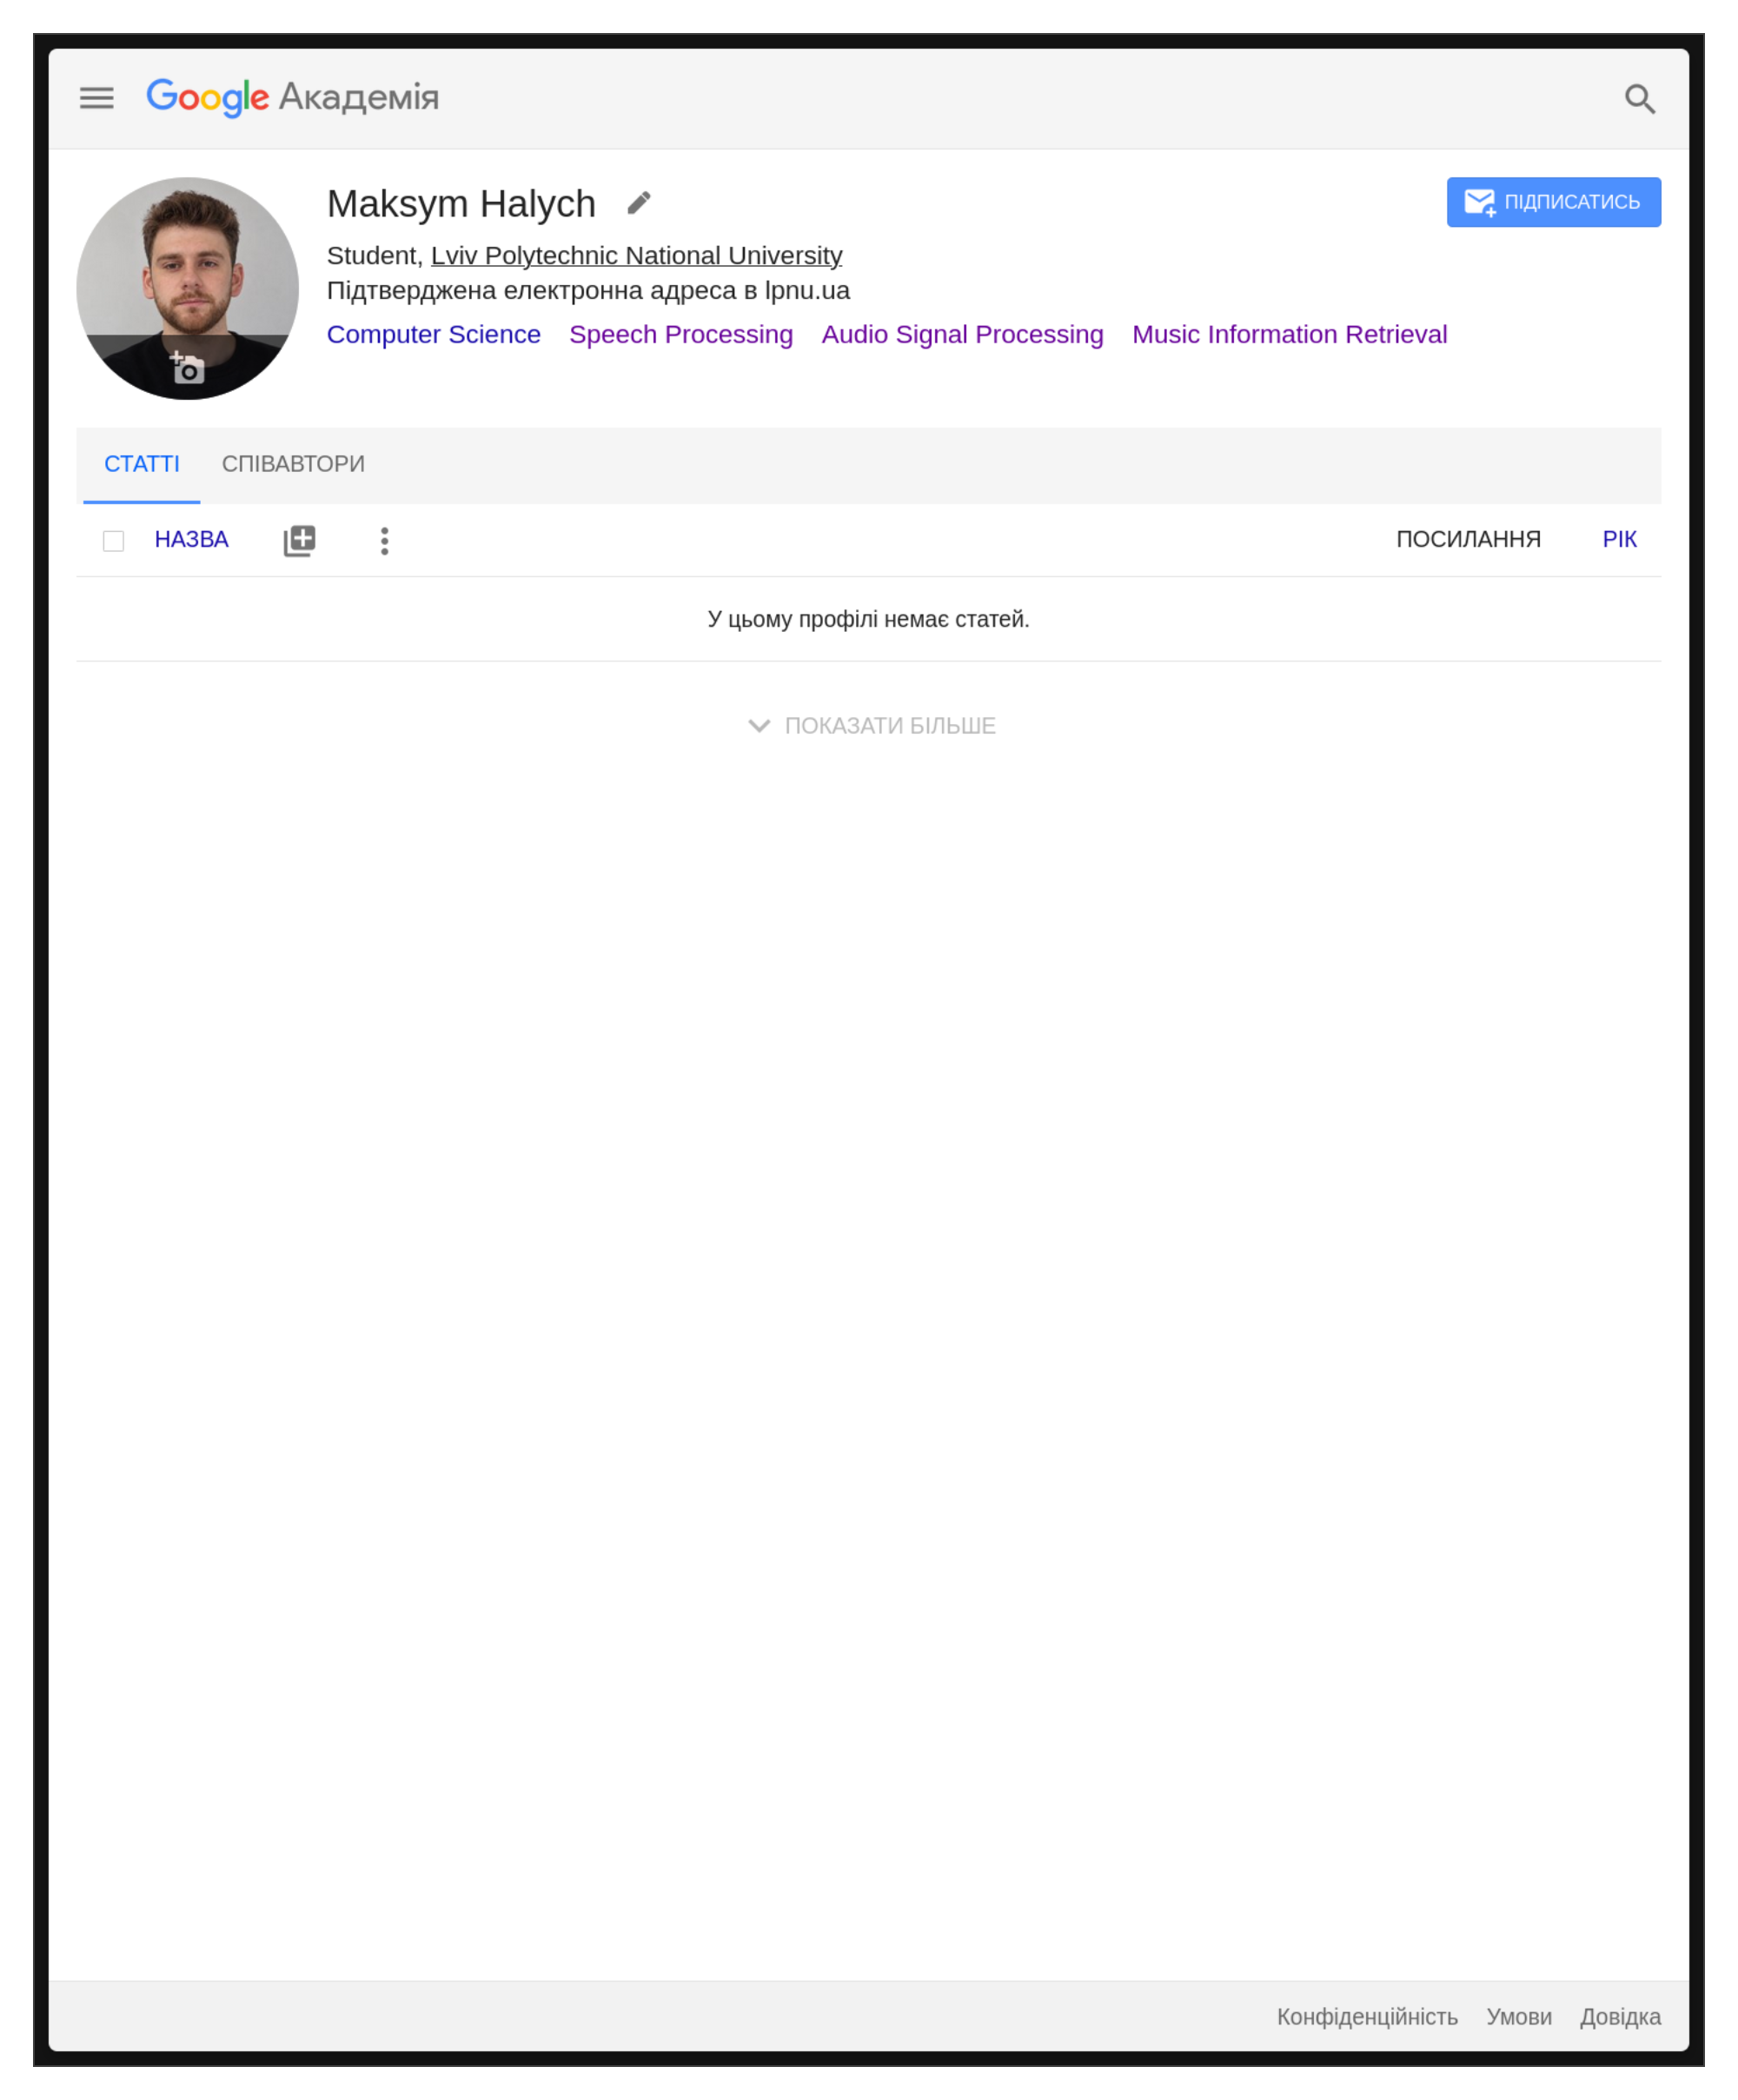
\includegraphics[width=\linewidth,trim={0 1516bp 0 0},clip]{scholar-profile}
  \caption{Заповнений профіль користувача у базі Google Scholar}
  \label{fig:scholar-profile}
\end{figure}

Профіль активовано підтвердженням корпоративної поштової адреси: на сторінці
профілю (рисунок~\ref{fig:scholar-profile}) під назвою установи відображається
позначка «Підтверджена електронна адреса в lpnu.ua». Саме вона робить профіль
видимим у результатах пошуку авторів і підтверджує приналежність автора до
Університету.

Майстер створення профілю вимагає долучити щонайменше одну публікацію, тому,
згідно з вказівками методичних рекомендацій, під час реєстрації до профілю
було додано сторонню публікацію, а одразу після створення профілю її
вилучено. Тому вкладка \textit{Статті} порожня — профіль не містить робіт,
які не належать автору.

\subsection{Web of Knowledge}

Реєстрацію на пошуковій платформі Web of Science (Web of
Knowledge)~[\ref{bib:wos-db}] на момент складання звіту не виконано.
Доступ до бази передплачено Міністерством освіти і науки України за запитом
Національного університету «Львівська політехніка» лише для працівників
і студентів Університету, і платформа розпізнає цю передплату за IP-адресою
відвідувача. Тому створити обліковий запис можна лише з комп'ютера,
під'єднаного до мережі Університету; корпоративна поштова адреса в домені
\texttt{lpnu.ua} сама собою цієї умови не замінює.

Такий порядок підтверджено на консультації до практичної роботи: реєстрацію
слід виконувати з комп'ютера Університету, а за відсутності доступу —
зазначити це у звіті й зареєструватися за першої нагоди. Саме так і вчинено:
крок відкладено до появи доступу до мережі Університету, після чого обліковий
запис буде створено за інструкцією користувача~[\ref{bib:wos-manual}]. Це
потрібно зробити до наступних практичних робіт, які спираються на цей запис.

Для подальшої роботи з платформою слід також
врахувати обмеження на періодичність входу: реєстрація надає доступ до
Web of Science з будь-якої IP-адреси через логін і пароль, однак раз на чотири
місяці необхідно зайти в систему з комп'ютера організації, яка передплатила
доступ, інакше авторизація перестає працювати.

\subsection{Scopus}

Нового користувача у наукометричній базі Scopus~[\ref{bib:scopus-db}]
зареєстровано заповненням форми, що з'являється після натискання кнопки
\textit{Create account}. Як і в попередньому випадку, використано корпоративну
поштову адресу \texttt{@lpnu.ua}, оскільки доступ до більшості інструментів
бази надається лише передплатникам~[\ref{bib:scopus-guide}].

Різницю у вигляді сторінки до та після входу в систему наведено на
рисунку~\ref{fig:scopus-login}: до логування бічна панель облікового запису
пропонує лише посилання \textit{Create account} та \textit{Sign in}, а після
нього — відображає ім'я користувача, корпоративну поштову адресу, розділ
\textit{My Scopus Preview} та команду виходу з системи.

% Обидва знімки — на всю сторінку, а змістовна тут лише бічна панель праворуч,
% тому беремо її виріз (1 px = 1 bp, див. коментар до scholar-profile) і
% обмежуємо висоту: два зображення на повну ширину в один [H]-рисунок не
% вміщаються у сторінку, і float змушує LaTeX крутити порожні сторінки без кінця.
% Панелі стоять поруч, бо порівнюються саме між собою, і виріз у них однаковий
% (950x1336 px) — тільки так вони мають однаковий розмір на сторінці. Висоту
% задає довша панель «б»: обрізати її до висоти «а» означало б втратити рядок
% «Sign out», а він тут і є доказом входу в систему. У «а» натомість лишається
% порожнє місце знизу — меню до логування справді коротше.
\begin{figure}[H]
  \centering
  \begin{minipage}[t]{0.46\linewidth}
    \centering
    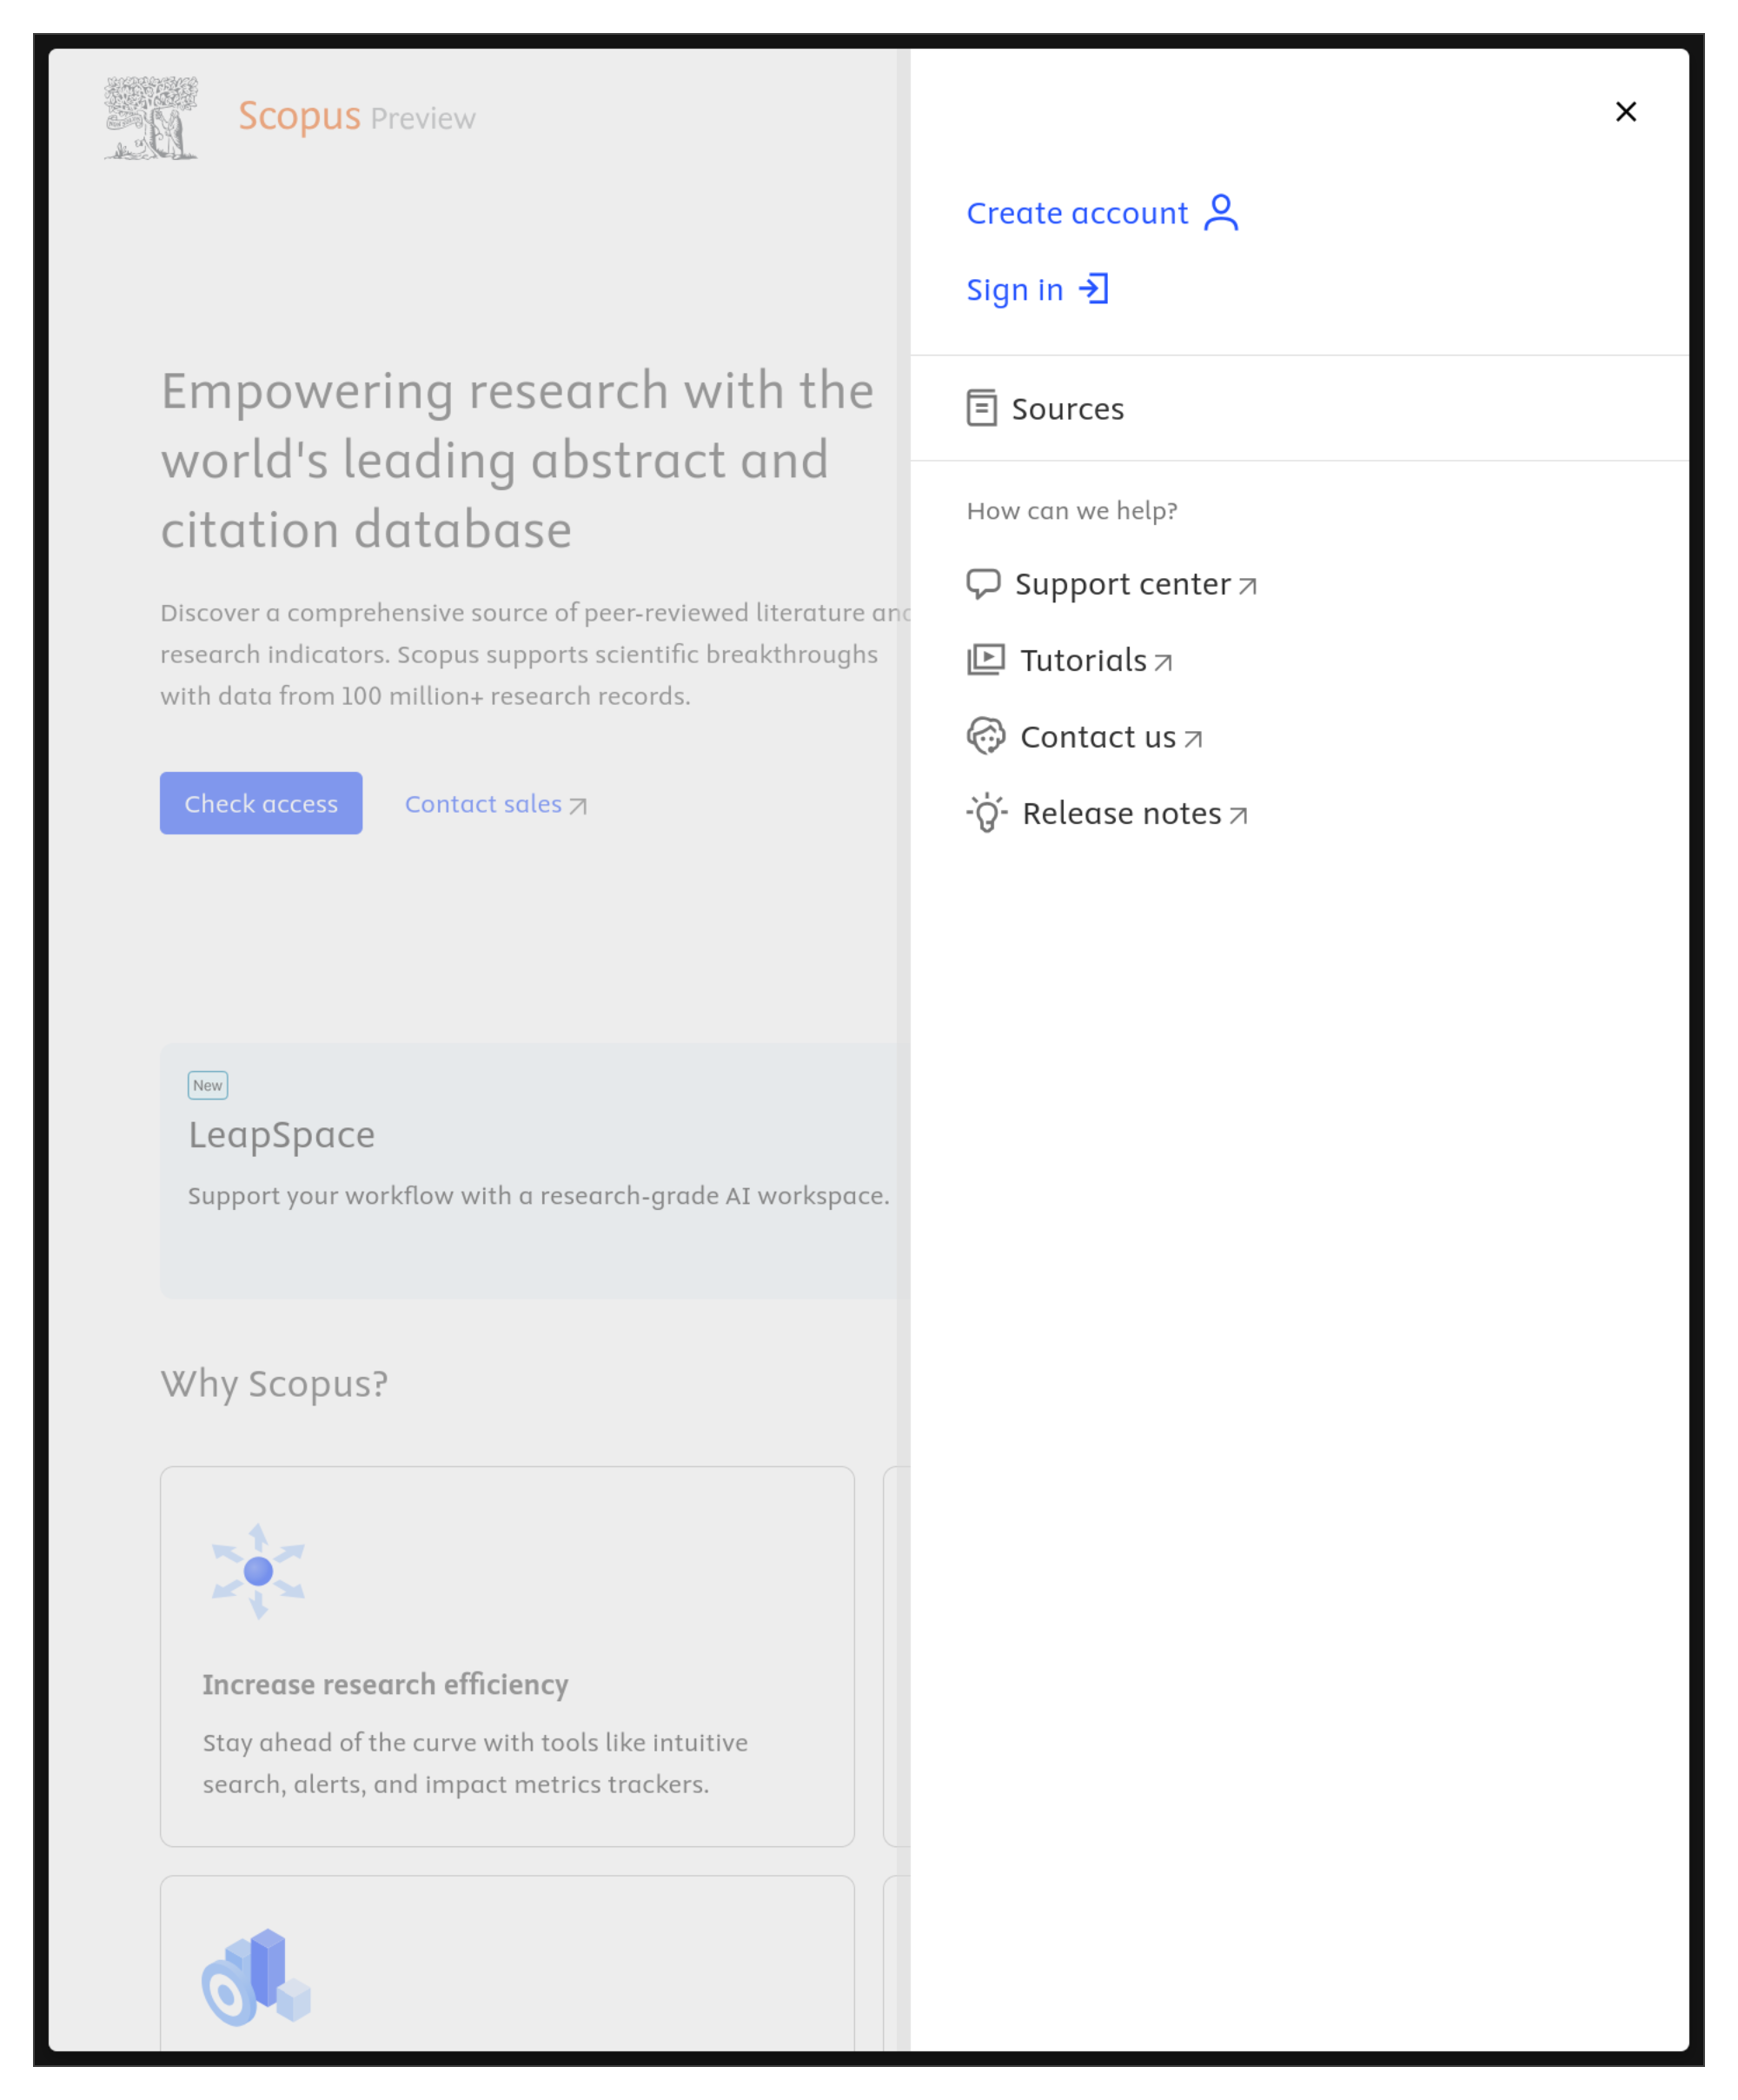
\includegraphics[width=\linewidth,trim={1050bp 1080bp 0 0},clip]{scopus-before-login}\\[6pt]
    а)
  \end{minipage}\hfill
  \begin{minipage}[t]{0.46\linewidth}
    \centering
    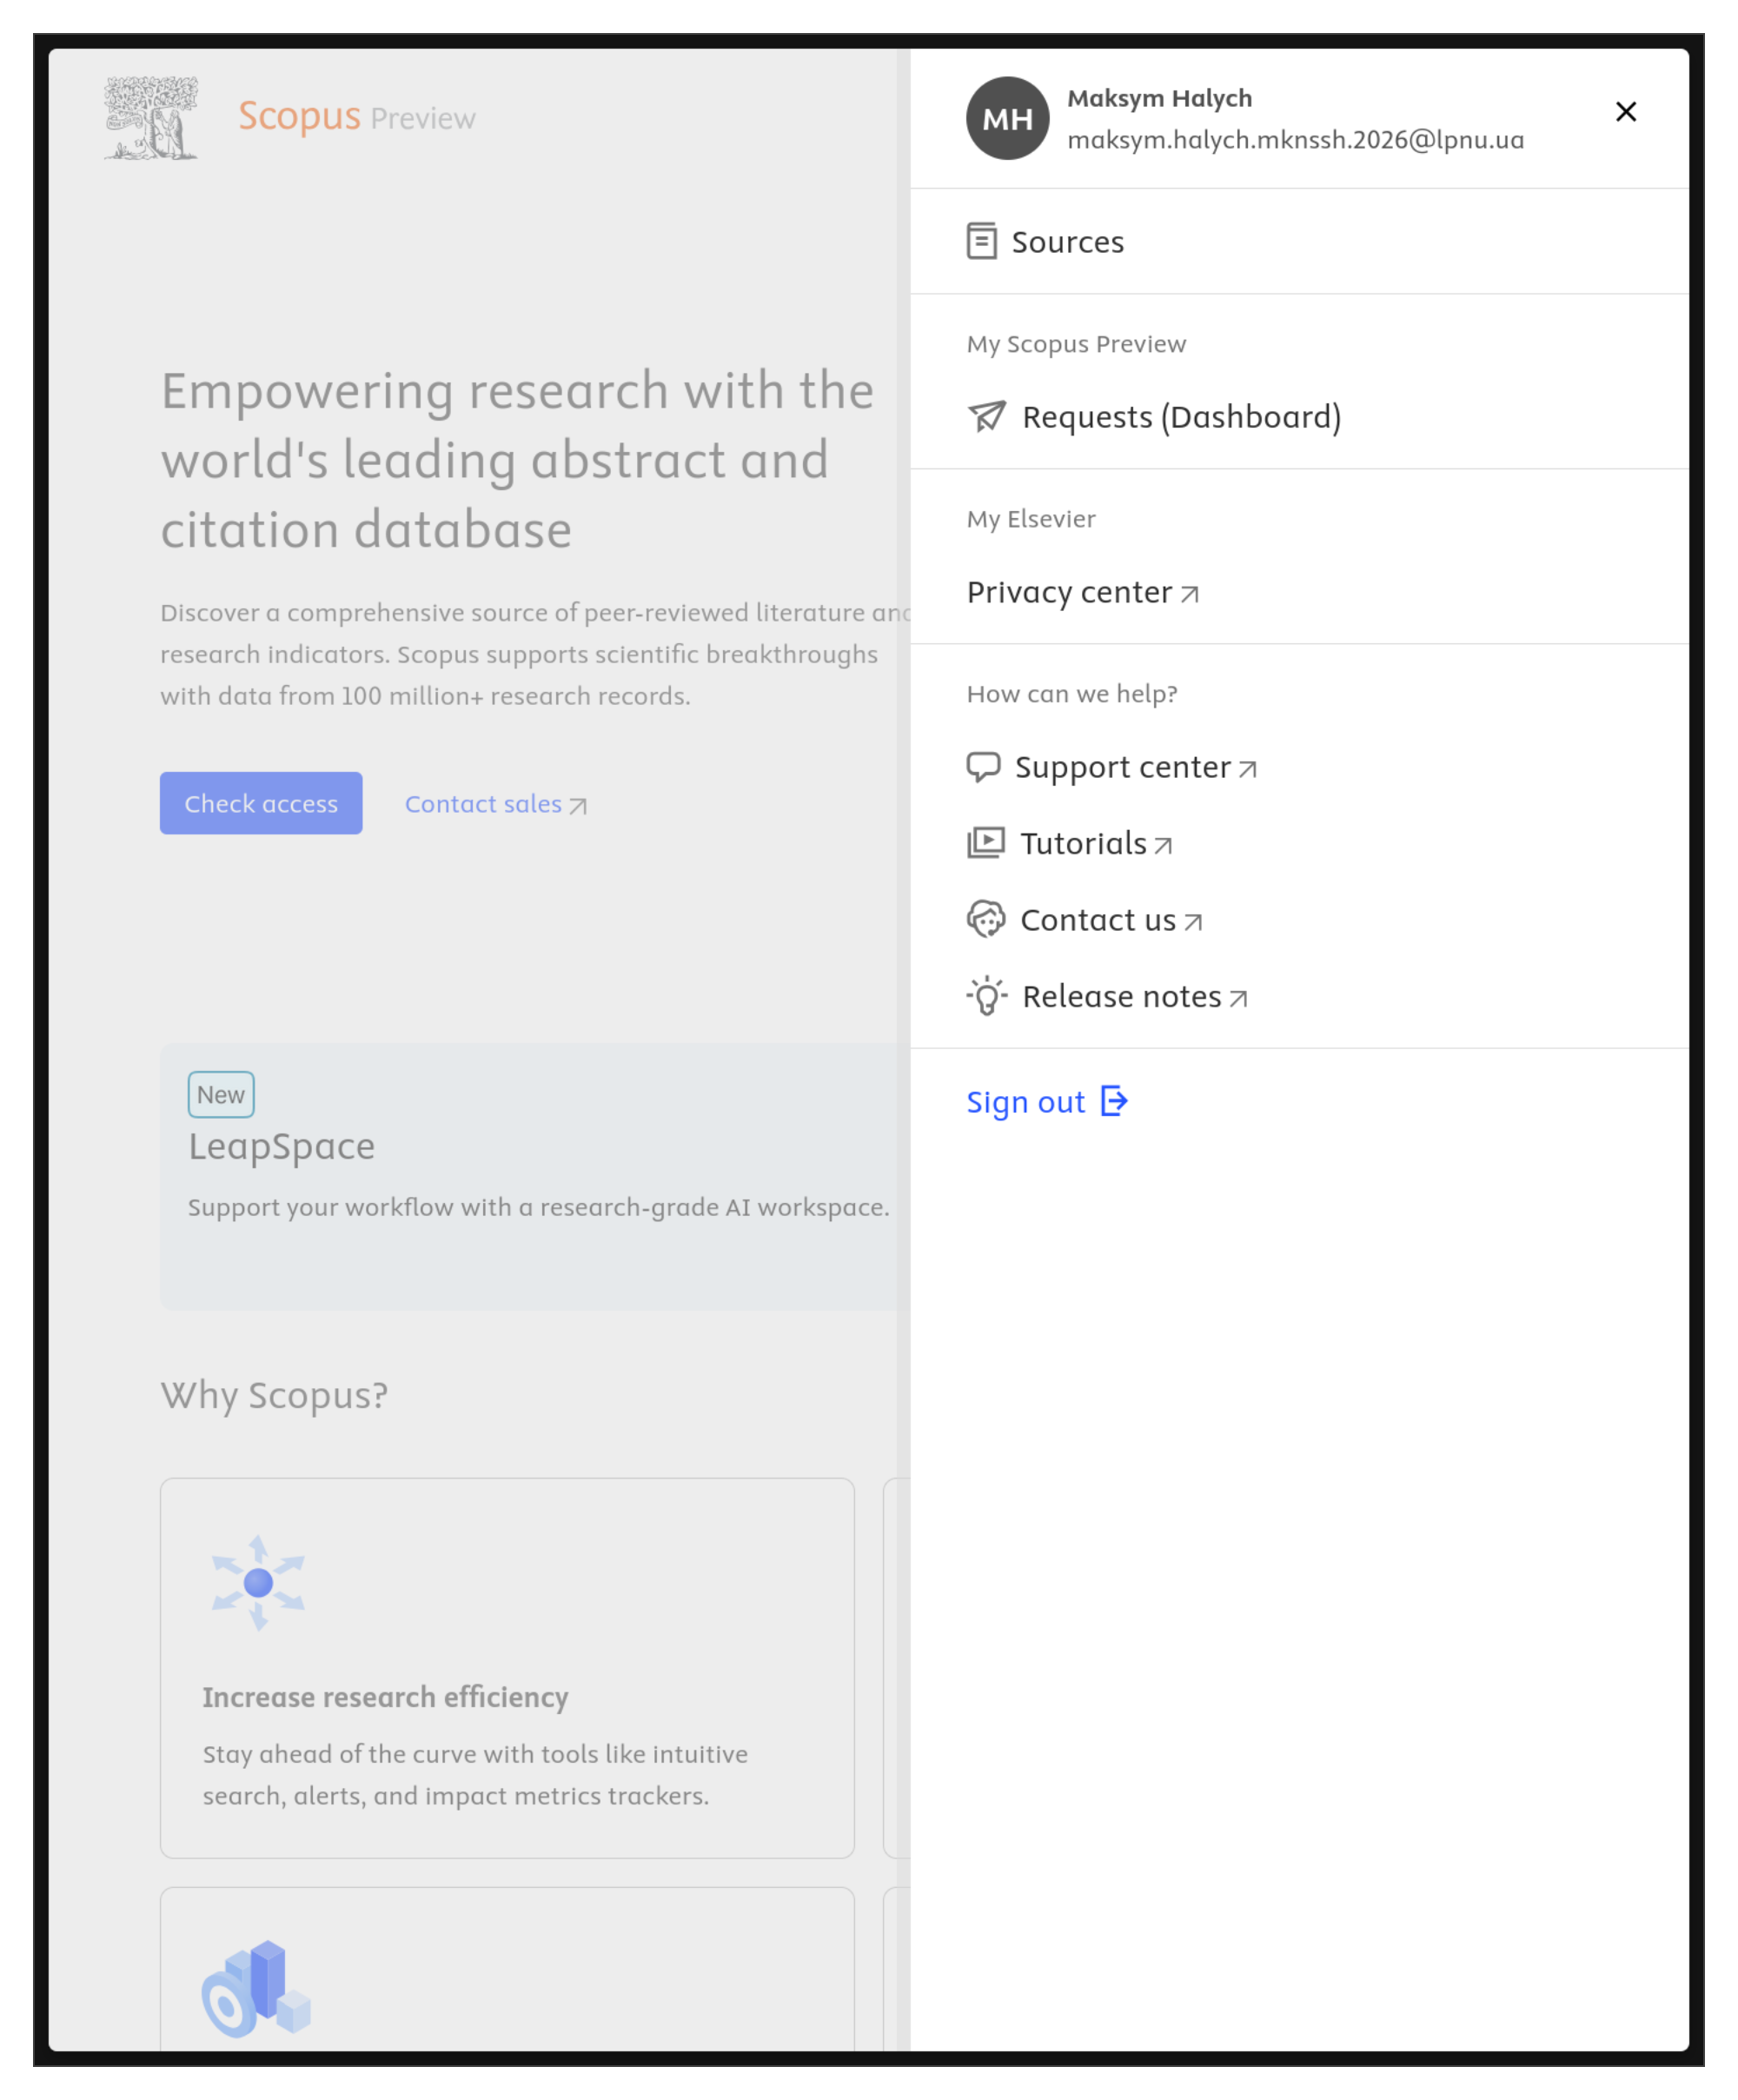
\includegraphics[width=\linewidth,trim={1050bp 1080bp 0 0},clip]{scopus-after-login}\\[6pt]
    б)
  \end{minipage}
  \caption{Вигляд бічної панелі облікового запису бази Scopus:
  а)~до логування, б)~після логування у систему}
  \label{fig:scopus-login}
\end{figure}

Варто зауважити, що обидва знімки зроблено в режимі \textit{Scopus Preview} —
саме його бачить користувач поза передплатою. Корпоративна адреса сама собою
повного доступу не відкриває: його надає IP-адреса мережі Університету або
вхід через інституційну автентифікацію, тож для роботи з повним набором
інструментів бази вхід слід виконувати з мережі Університету.

Слід розрізняти дві різні сутності: обліковий запис користувача, створений
реєстрацією, та профіль автора, який Scopus створює автоматично для осіб,
що мають проіндексовані в базі публікації. Ці дві сутності між собою не
пов'язані. Для перевірки наявності автоматично створеного профілю використано
форму пошуку за ПІБ (\textit{Authors}); результат пошуку наведено на
рисунку~\ref{fig:scopus-author}. За запитом «Halych, Maksym» база повернула
\textbf{0 author results}, тобто автоматично створеного профілю автора не
існує — публікацій, проіндексованих у Scopus, немає.

\begin{figure}[H]
  \centering
  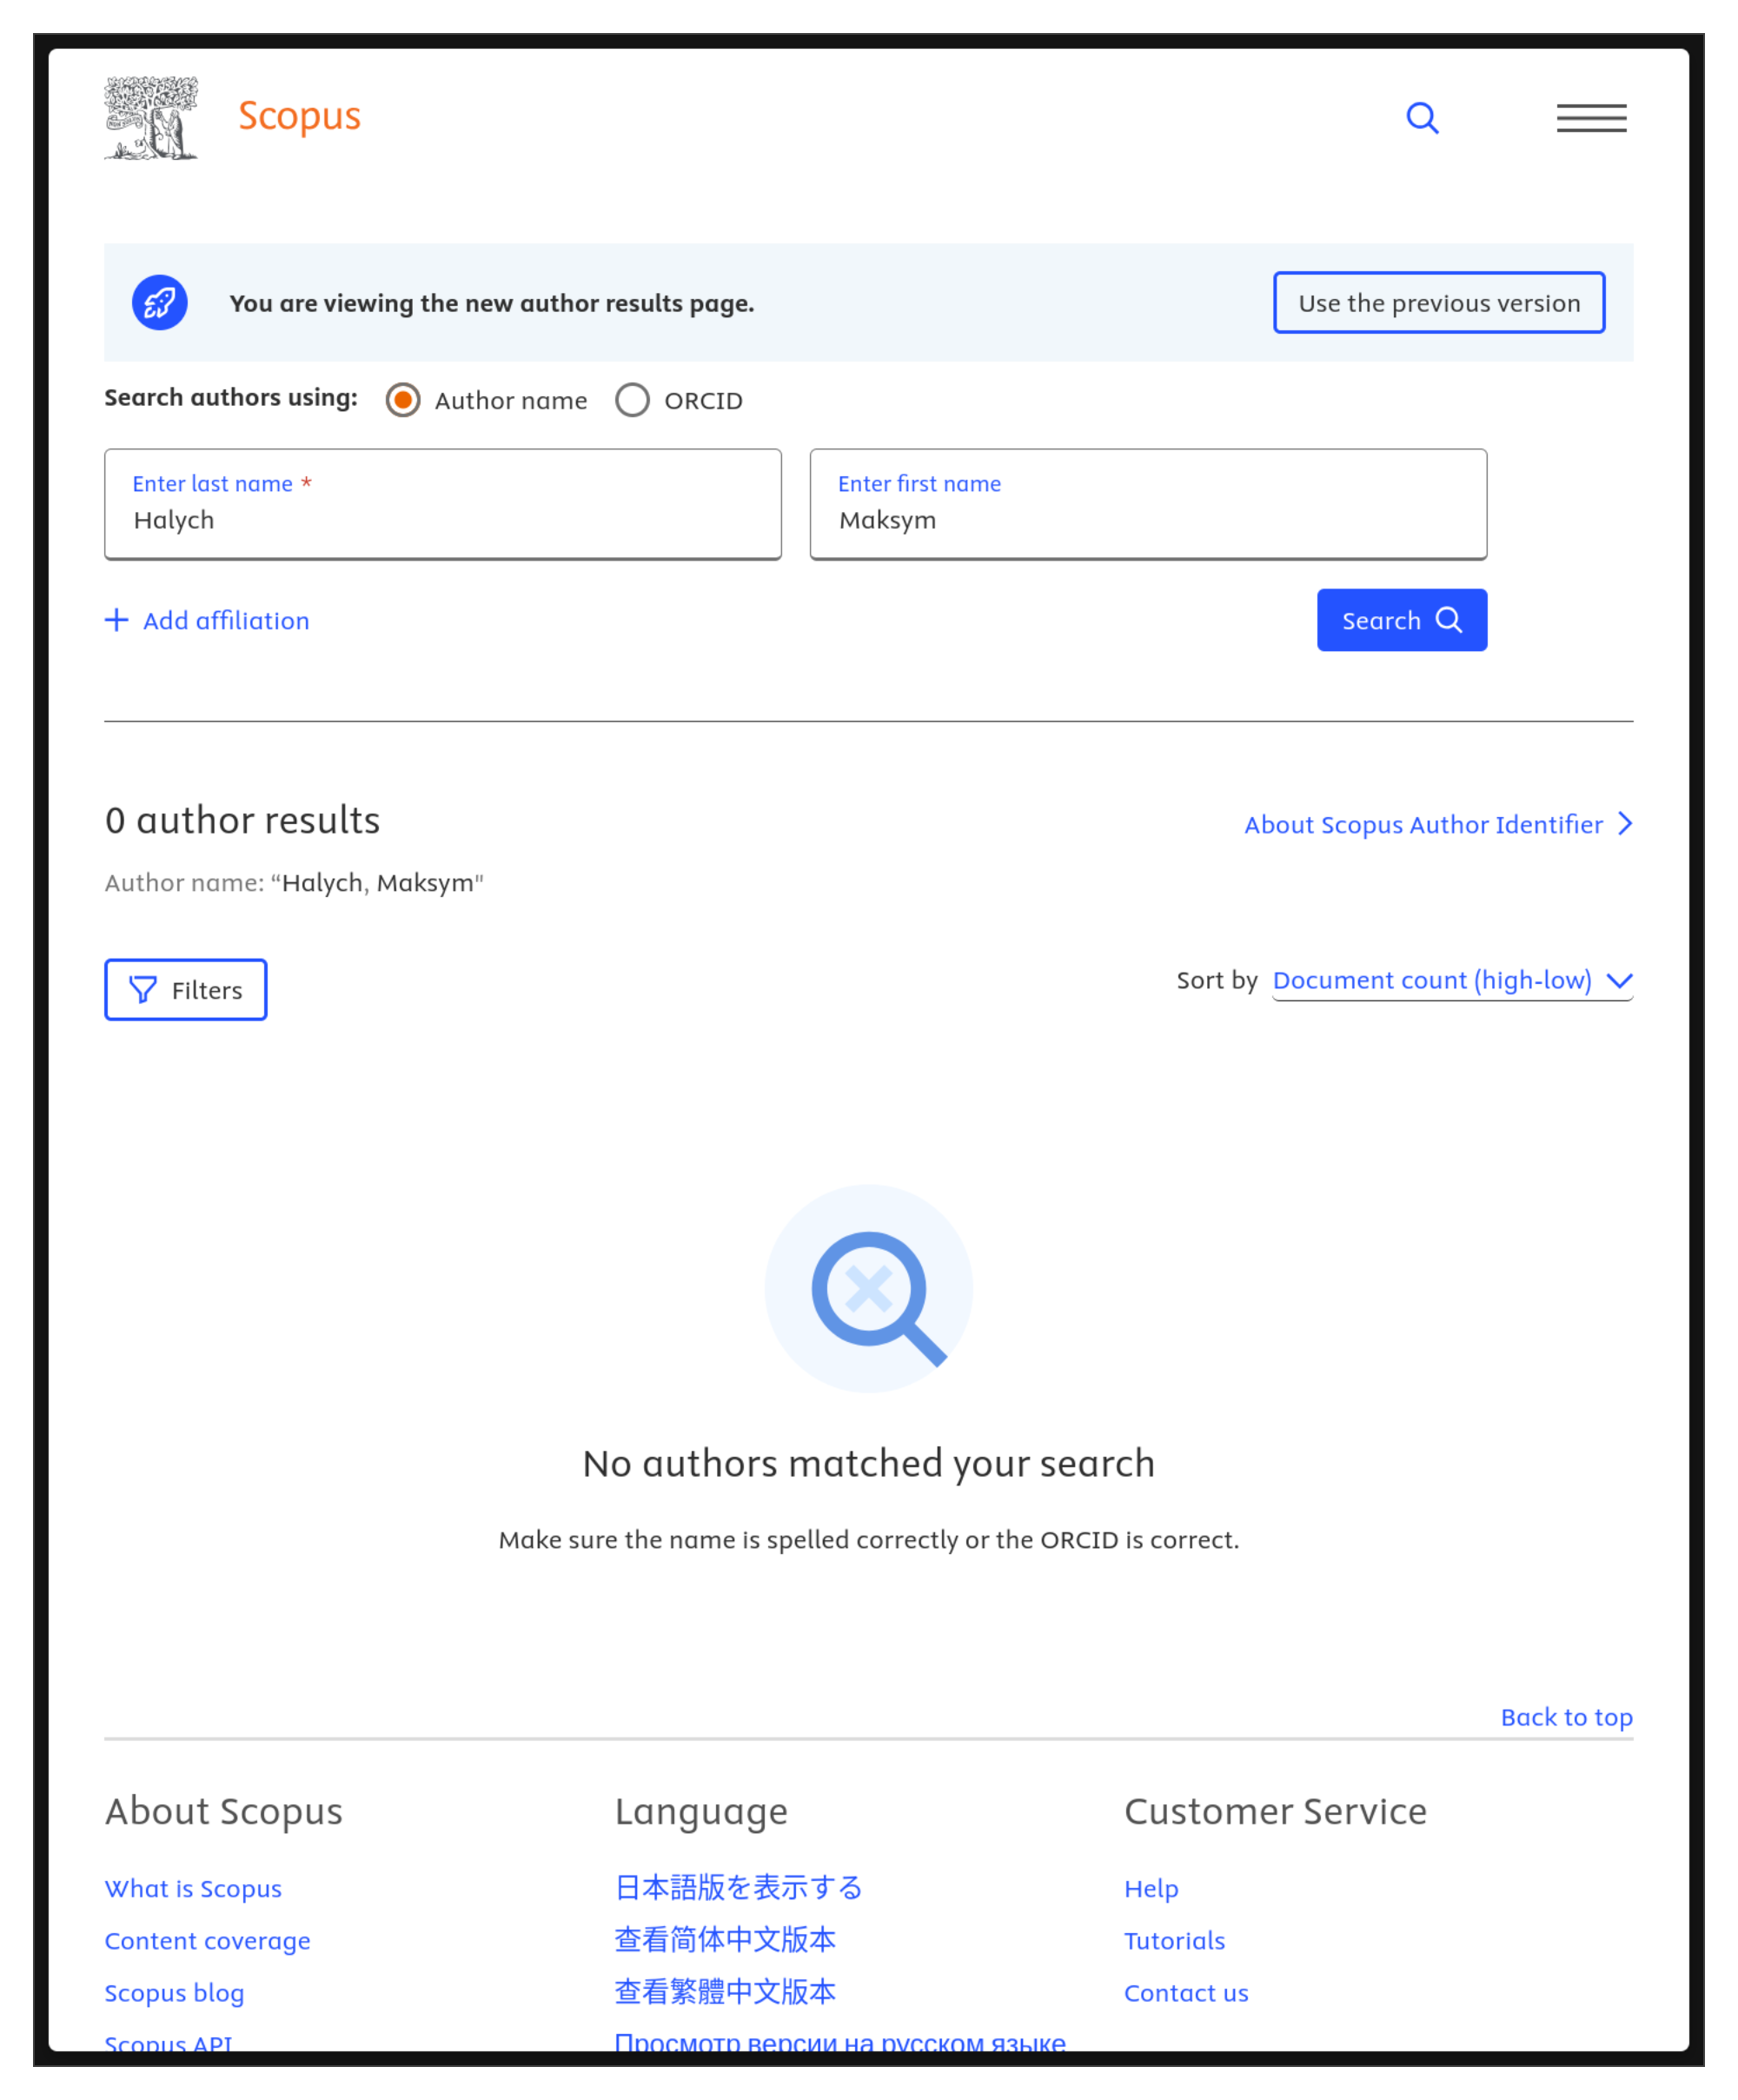
\includegraphics[width=\linewidth]{scopus-author-search}
  \caption{Результат пошуку автора за ПІБ у базі Scopus}
  \label{fig:scopus-author}
\end{figure}

\subsection{ORCID}

Обліковий запис ORCID~[\ref{bib:orcid-db}] створено за
рекомендаціями~[\ref{bib:orcid-manual}]: заповнено реєстраційну форму,
підтверджено поштову адресу й активовано запис, а видимість даних профілю
встановлено публічною (\textit{Everyone}) — без цього ідентифікатор не
виконує своєї основної функції, адже зв'язок автора з його роботами має
бути перевірним ззовні.

Запису присвоєно ідентифікатор \href{https://orcid.org/\OrcidID}{\OrcidID}.
Заповнено обов'язкові для роботи атрибути: місце навчання
(\textit{Education and qualifications}) — Lviv Polytechnic National University,
кафедра систем штучного інтелекту, бакалаврат 2022--2026~рр.; та місце праці
(\textit{Employment}) — за відсутності місця праці вказано Університет,
із вереснем 2026~р. як початком. Корпоративну адресу в домені \texttt{lpnu.ua}
підтверджено, що видно в розділі \textit{Emails \& domains}. Загальний вигляд
облікового запису наведено на рисунку~\ref{fig:orcid-record}.

\begin{figure}[H]
  \centering
  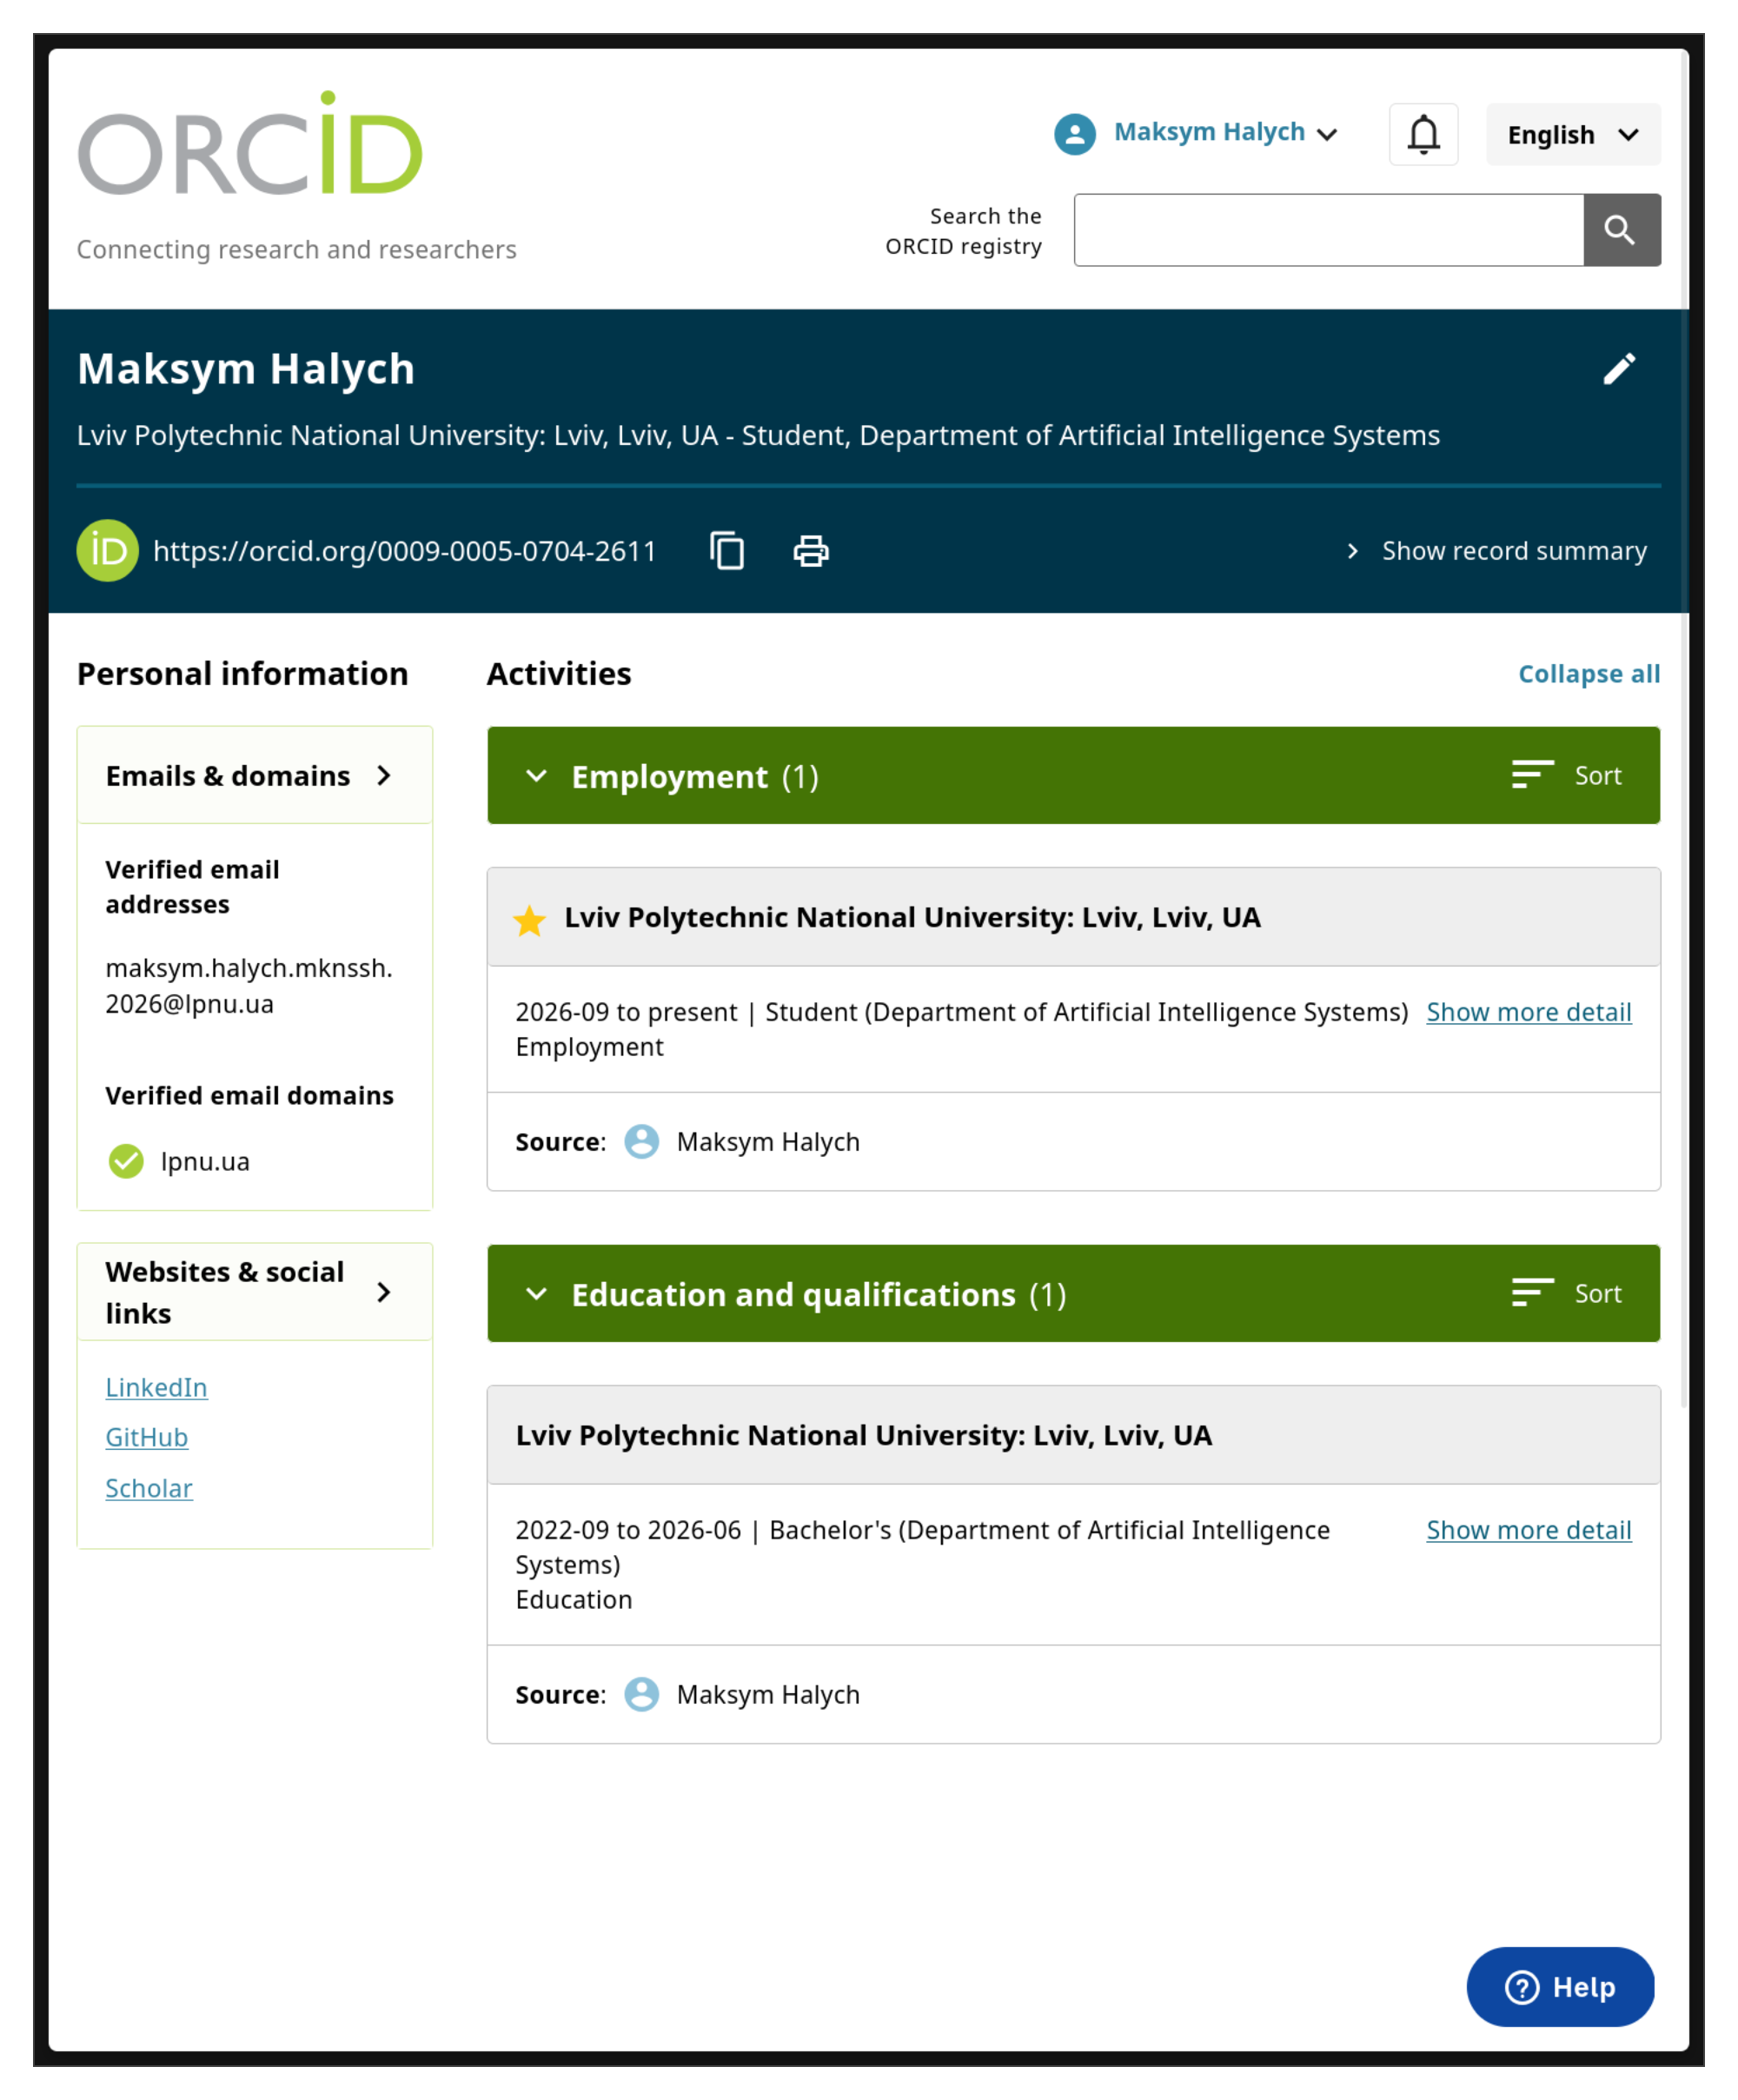
\includegraphics[width=\linewidth]{orcid-record}
  \caption{Загальний вигляд облікового запису ORCID із заповненими розділами
  \textit{Employment} та \textit{Education and qualifications}}
  \label{fig:orcid-record}
\end{figure}

У поле \textit{Websites \& Social Links} долучено три посилання, видимі
в лівій колонці рисунка~\ref{fig:orcid-record}: на профіль у Google Scholar,
на профіль у соціальній мережі LinkedIn і додатково на профіль у GitHub.
Саме цей розділ перетворює ORCID на точку входу до решти профілів автора:
один ідентифікатор веде до всіх його наукометричних і професійних сторінок.

Автоматично створеного профілю автора у базі Scopus на момент виконання
роботи не існує, оскільки проіндексованих у ній публікацій немає. Відповідно,
зв'язування профілів Scopus і ORCID не виконувалося; цю операцію буде
здійснено після першої публікації, долученої до бази.

\section{Результати}

У результаті виконання роботи створено й наповнено три профілі: у базах
Google Scholar і Scopus та в реєстрі ідентифікаторів ORCID. Реєстрацію
у Web of Knowledge відкладено до появи доступу з мережі Університету
(пункт~\ref{concl:wos} висновків). QR-код створеного облікового запису ORCID
наведено на рисунку~\ref{fig:orcid-qr}.

\begin{figure}[H]
  \centering
  
\includegraphics[width=0.35\linewidth]{orcid-qr}
  \caption{QR-код облікового запису ORCID}
  \label{fig:orcid-qr}
\end{figure}

Ідентифікатори автора у створених профілях подано в таблиці~\ref{tab:ids};
ідентифікатори є активними гіперпосиланнями на відповідні профілі.

\begin{table}[H]
\caption{Мій ідентифікатор ORCID та профіль у Google Scholar}
\label{tab:ids}
\begin{tabularx}{\linewidth}{|c|X|l|}
\hline
\textbf{№} & \textbf{Наукометрична база/сервіс} & \textbf{Ідентифікатор автора} \\
\hline
1 & Google Scholar &
\href{https://scholar.google.com/citations?user=\ScholarID}{\ScholarID} \\
\hline
2 & ORCID &
\href{https://orcid.org/\OrcidID}{\OrcidID} \\
\hline
\end{tabularx}
\end{table}

\section{Висновки}

У ході практичної роботи створено й наповнено профіль користувача у базі
Google Scholar, обліковий запис у базі Scopus та обліковий запис у реєстрі
ORCID, а також розібрано принципи формування наукометричних рейтингів
у Scopus і Google Scholar. Реєстрацію у Web of Knowledge відкладено
з причин, описаних нижче.

\begin{enumerate}[ref=\arabic*]
\item Створено та активовано профіль у Google Scholar із заповненими
атрибутами й підтвердженою корпоративною поштовою адресою. Сторонню
публікацію, додану майстром реєстрації як обов'язкову, після створення
профілю вилучено, тому профіль містить лише роботи автора.

\item\label{concl:wos} Реєстрацію у Web of Knowledge не виконано, і причина
не технічна, а організаційна: платформа зіставляє відвідувача з передплатою
Університету за IP-адресою, тому створити обліковий запис можна лише
з комп'ютера, під'єднаного до мережі Університету. Поза нею потрібної форми
просто не отримати, і корпоративна поштова адреса цього не змінює. Спосіб
виходу із ситуації один — виконати реєстрацію з мережі Університету, що й
буде зроблено за першої нагоди, оскільки обліковий запис потрібен для
наступних практичних робіт.

\item Зареєстровано користувача у Scopus із корпоративної адреси
\texttt{@lpnu.ua}. З'ясовано, що сама собою корпоративна адреса повного
доступу не відкриває: інструменти бази доступні передплатникам, і поза
мережею Університету база працює в обмеженому режимі \textit{Scopus Preview}.

\item Створено, активовано та зроблено публічно видимим обліковий запис
ORCID із заповненими місцем навчання й праці та посиланнями на профіль
у Google Scholar і соціальній мережі.

\item Розмежовано два поняття, які легко сплутати: обліковий запис
користувача бази та профіль автора. Перший створює сам користувач
реєстрацією, другий Scopus формує автоматично за наявності проіндексованих
публікацій, і між собою вони не пов'язані.

\item Щодо формування рейтингу: Google Scholar обчислює \textit{h}-індекс
та \textit{i10}-індекс за всіма проіндексованими цитуваннями, включно
з препринтами, тезами й матеріалами конференцій, тому його показники
систематично вищі. Scopus рахує \textit{h}-індекс лише за публікаціями
у виданнях, долучених до бази, тому його значення нижче, але зіставне між
авторами. Ширше покриття Google Scholar дається ціною слабшої фільтрації
джерел, і це робить показники двох баз непорівнюваними безпосередньо.

\item Практичний сенс виконаної роботи полягає в тому, що ORCID стає
постійним ідентифікатором автора, незалежним від написання прізвища різними
мовами й від зміни місця праці, та єдиною точкою входу до решти профілів.
Це знімає проблему неоднозначної ідентифікації дослідників з однаковими
або поширеними прізвищами, яка і була причиною появи ORCID.
\end{enumerate}

\section{Список використаної літератури}

\begin{enumerate}[label=\arabic*., ref=\arabic*, itemsep=6pt]
\item\label{bib:scholar} Пошукова та наукометрична система Google Scholar
[Електронний ресурс]. --- Режим доступу:
\url{https://scholar.google.com/?hl=uk} (дата звернення: 10.02.2026).

\item\label{bib:scholar-db} Веб-адреса бази даних Google Scholar
[Електронний ресурс]. --- Режим доступу: \url{https://scholar.google.com/}
(дата звернення: 10.02.2026).

\item\label{bib:wos-manual} База даних Web of Science. Версія 5.22.
Інструкція користувачу [Електронний ресурс]. --- Режим доступу:
\url{http://www.nbuv.gov.ua/sites/default/files/basicpage_files/201705_basicpage_files_mat/instruction.pdf}
(дата звернення: 10.02.2026).

\item\label{bib:wos-db} Веб-адреса бази даних Web of Science
[Електронний ресурс]. --- Режим доступу:
\url{https://www.webofknowledge.com} (дата звернення: 10.02.2026).

\item\label{bib:scopus-guide} Scopus --- докладна інструкція для вченого
[Електронний ресурс]. --- Режим доступу:
\url{https://ua.publ.science/uk/blog/scopus---podrobnaya-instruktsiya-dlya-uchenogo}
(дата звернення: 10.02.2026).

\item\label{bib:scopus-db} Веб-адреса бази даних Scopus
[Електронний ресурс]. --- Режим доступу:
\url{https://www.scopus.com/search/form.uri?display=basic}
(дата звернення: 10.02.2026).

\item\label{bib:orcid-manual} Рекомендації. ORCID та Researcher ID.
Як зареєструватися та здійснювати обмін інформацією [Електронний ресурс].
--- Режим доступу:
\url{https://stu.cn.ua/wp-content/uploads/2021/04/orcid_instructions.pdf}
(дата звернення: 10.02.2026).

\item\label{bib:orcid-db} Веб-адреса інформаційної системи ідентифікації
науковців ORCID [Електронний ресурс]. --- Режим доступу:
\url{https://orcid.org/} (дата звернення: 10.02.2026).
\end{enumerate}

\end{document}
